

\subsubsection{Introduction}
Every day we make predictions based on our personal subjective experiences.
Our predictions about durations or extent of everyday phenomena such as human
 life spans and the box-office take of movies are based on an optimal
Bayesian model\citep{OptimalPredEveryDay}.
Human perceptions, memory, inferring a 3D structure from a 2D structure,
judging when a particular fact is likely to happen in the future are also
 based on approximate statistical inference.

It is possible then, that we use Bayesian inference when bidding on the final
 price of an auction.
There are 3 main type of auctions known in literature\citep{AuctionTypes}:
\begin{itemize}
 \item First Price Auction: an auction in which the bidder who submitted the
 highest bid is awarded the object being sold and pays a price equal to the amount bid.

 \item Second Price Auction: an auction in which the bidder who submitted the
 highest bid is awarded the object being sold and pays a price equal to the second highest amount bid.

 \item English Auction: a type of sequential second price auction  in which an
 auctioneer directs participants to beat the current, standing bid. New bids must
 increase the current bid by a predefined increment. The auction ends when no
 participant is willing to outbid the current standing bid. Then, the participant
 who placed the current bid is the winner and pays the amount bid.
\end{itemize}
% 
First and Second Price Auctions follow a Bayesian Nash Equilibrium, but there are
 no models of English price auction based on ABM (agent based model) where agents
 make prediction about the final price and also about other's expectations.

I assume that in English price auctions, players uses Bayesian inference to
 estimate the final price $v_{final}$ of an auction $b$. For clarity of notation
 I will use $p$ to indicate probabilities, $v$ to indicate prices (values),
$a_i$ to indicate an agent with $i=1,...,n$, $b$ to indicate an auction.
The task of the agent $\forall a_i$ is to estimate $v_{final}$ from the
current price $v$ of the auction $b$.
The Bayesian predictor computes a probability distribution over $v_{final}$
given $v$, by applying the Baye's rule:
\begin{equation}
 p(v_{final}|v)\propto p(v|v_{final})p(v_{final})
\end{equation}
The conditioned probability of the event $v_{final}$ given the actual price $v$
 is proportional to likelihood $p(v|v_{final})$ and the prior probability $p(v_{final})$.
The likelihood is the probability of observing during an auction $b$ a bid of
 price $v$ given that the final price of the auction is $v_{final}$.
We assume that agents are equally likely to observe any price of an auction in the
 range $[0,v_{final}]$, which means using a uniform random sampling rate.
\begin{eqnarray}
p(v|v_{final})=1/v_{final},v<v_{final}\\
p(v|v_{final})=0,v>v_{final}
\label{bayes:eq:1}
\end{eqnarray}
The same assumption was also used in \citep{OptimalPredEveryDay} for the duration
 of life spans but also in Bayesian models of visual perception.
The prior probability $p(v_{final})$ models the agent's expectation about the
 final price of the auction $b$.
A statistical analysis of online ebay auctions shows that there are two main classes
 of final price distributions. A class of products -such as cars- follow a Gaussian
 distribution with mean $\mu$ and standard deviation $\sigma$ where others
-such as handy crafts- follow a gamma distribution with scale parameter $\theta$
and shape parameter $k$.
The difference in distribution could be caused by the fact that the price of
commodity gods such as cars can be assessed precisely, whereas for other niche
 gods the price distribution has a long tail due to over estimation.
Combining the prior with the likelihood according to Eq.\ref{bayes:eq:1} yields a
probability of $p(v_{final}|v)$ over all possible final prices for an auction
 with a current value of $v$.
A good guess for $v_{final}$ is thus the median of this distribution, called a
 Bayesian prediction function which estimates the final price of an auction
given the current price.
Every agent $a_i$ has thus a prediction function:
\begin{eqnarray}
Pred_{i}:v \rightarrow v_{final}
\end{eqnarray}
which allows the estimation of the final price of an auction given the current price.
Gaussian prior have non linear prediction functions, whereas Erlang priors have
 linear prediction functions.
Evert agent has also an expectation function:
\begin{eqnarray}
 Exp_{i,j}:v \rightarrow v_{final}
\end{eqnarray}
 which models the expectation that the agent $i$ has toward the prediction
function of the agent $j$.
The expectation function is computed by the agent during the auction and is a
point estimate of the others' prediction functions.
It also necessary to introduce an energy function $E_{i}: t \rightarrow p_{bid} $
 for every agent $i$ which models the risk associated with the bidding:
\begin{equation}
E_{i}=\frac{p_{max}}{1+exp(-m_{i} \cdot t)}
\end{equation}
where $p_{max}=1$ for normalization, $p_{bid}$ is the probability of bidding and
 $m_{i}$ is the sensitivity to the risk. The logit function is based on the typical
behaviour of online auctions where the rate of bidding is increasing toward the end
of the auction.
The energy function is essentially a reward signal similar to the one used in
the Q-learning learning agent.

\subsubsection{Virtual auction model}
In a virtual auction there are $N$ agents modelled as grey boxes.
Every agent $i=1,...,N$ has a prediction function $Pred_{i}$ and an expectation
 function $Exp_{i,j}$ with $i \neq j$.
Agents bid in sequence at regular intervals, the auction starts with an initial
price of 0 and stops after $T$ time steps.
At each time step the agent can decide whether to bid or not.
Every agent has equal buying power but could have different prediction functions
 according to their subjective knowledge (a priori distribution).
Each agent's goal is to win the bid, which means to predict or estimate the final
price of the bid according to the actual price. The disturbance is generated by
 other agents bidding in temporal sequence.
Agents are not allowed to communicate with external channels or to bid on
multiple auctions. Every auction is independent from each other and agents
learn from each auction experience.
As an explicative example I show that by choosing an Erlang prediction function
 (see Eq.\ref{eq:ErlangPred}) for $N=2$ agents without expectations, the time series
has a linear behaviour.
\begin{figure}[!htbp]
	\begin{center}
	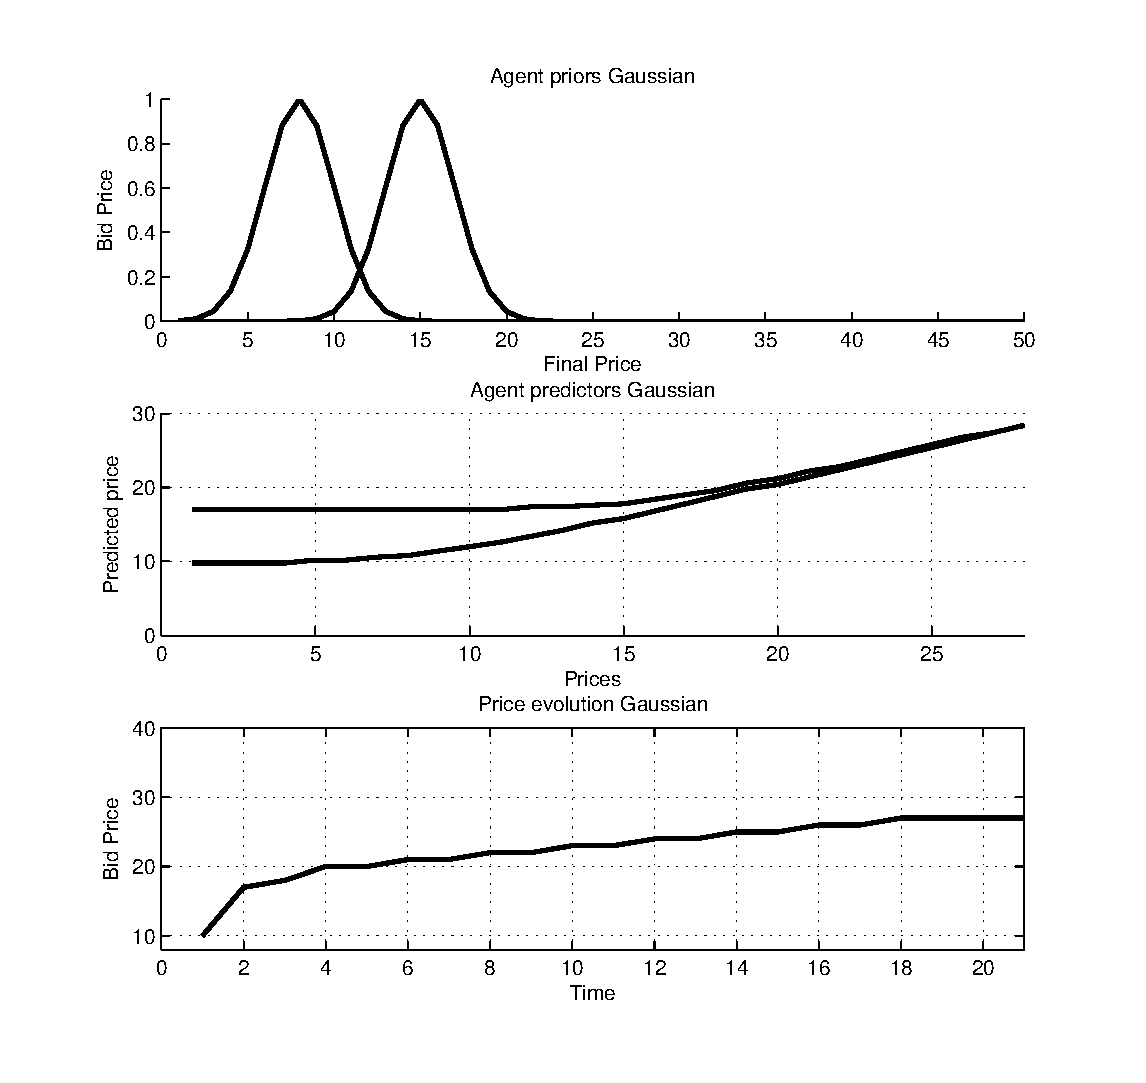
\includegraphics[width=0.8\textwidth]{economy/GaussianEvolution.eps}
	\end{center}
	\caption[Multi Agent Gaussian]{Two virtual agents using a Gaussian prediction function}
	\label{GaussianAuction}
\end{figure}
In the second example if I choose a Gaussian prediction function
(see Fig.\ref{GaussianNumericalPosterior}) for $N=2$ agents without expectations,
the time series has a non linear behaviour.
\begin{figure}[!htbp]
	\begin{center}
	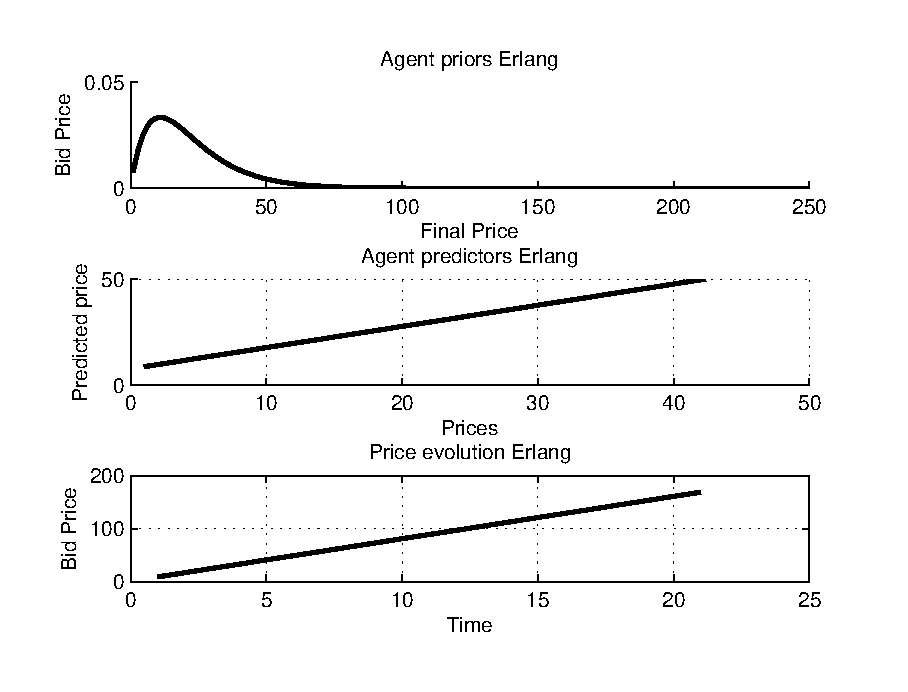
\includegraphics[width=0.8\textwidth]{economy/ErlangSymmetric.eps}
	\end{center}
	\caption[Multi Agent Erlang]{Two virtual agents using an Erlang prediction function.}
	\label{ErlangAuction}
\end{figure}


\subsubsection{Discussion}

The model could be validated in accuracy over 2 parameters:
\begin{itemize}
\item final price prediction: prediction of the final price of an item when $N$
      human agents are bidding
\item time series similarity: trajectories of price evolution during bidding
\end{itemize}
Firstly one could measure the ability of the model to predict the final price
of an an auction by only providing the parameter $N$ and the coefficient
of dissimilarity between players $C$.
In particular given a new ebay auction where we only know the initial price and
 the number of bidders the model would predict the final price with a confidence
 interval of $\xi$.

Secondly one could measure the similarity of the trajectories produced by the
 model with real online auctions.
For this purpose, it is possible to collect auction data from Ebay,
one of the biggest online auction websites.
The data should be filtered to remove multiple bidders (the same player bids on
different auctions) and automated ``snipers`` ( softwares agent that bid at the
last moment before an auction closes).
It should not be necessary to filter the automatic bidding function:
a player can set a limit budget and the ebay system will incrementally bid until
 the limit is reached.
These are special cases of bidding behaviour which are not reproduced in the model:
\begin{itemize}
 \item multi bid: agents bets on parallel auctions thus maximising their
chances of winning the same item at lower prices
 \item uniform sampling of prices
 \item offline learning: during the auction, the agents uses the static predictive function
 and expectations, they only update their a priori distribution between bidding
 sessions
\end{itemize}

A priory biasing is an important factor for symmetry breaking, when all the players
 have the same subjective knowledge the time series are linear, in the case of Erlang
 distributions and to some extent in the Gaussian distributions.
But expectations will play an important role in generating the necessary
dynamic during the bidding process.
In summary, this simplified learning model could predict the outcome of ebay
auctions and therefore can be extended to similar economic games where prediction
is essential like the stock market. 